\documentclass[11pt]{article}

\usepackage[margin=1in]{geometry}
\usepackage[T1]{fontenc}
\usepackage[utf8]{inputenc}
\usepackage{times}
\usepackage{amsmath,amssymb}
\usepackage{booktabs}
\usepackage{graphicx}
\usepackage{subcaption}
\usepackage[round,authoryear]{natbib}
\usepackage[colorlinks=true,linkcolor=blue,citecolor=blue,urlcolor=blue]{hyperref}
\usepackage{microtype}
\usepackage{url}

\newcommand{\Tel}{\mathrm{Tel}}
\newcommand{\Teo}{\mathrm{Teo}}
\newcommand{\Jaccard}{J}
\newcommand{\Align}{A}



\title{Quantitative Re-analysis of Published Top-Down Proteoform Counts Reveals Regional Separation in the Adult Zebrafish Brain}
\author{Anonymous Authors}
\date{}
\hypersetup{
  pdftitle={Quantitative Re-analysis of Published Top-Down Proteoform Counts Reveals Regional Separation in the Adult Zebrafish Brain},
  pdfauthor={Anonymous Authors}
}

\begin{document}
\maketitle

\begin{abstract}
Adult zebrafish telencephalon and optic tectum stand on opposite sides of the forebrain-visuomotor divide, yet it has remained unclear how sharply that difference appears at the proteoform level. We analyzed the region-resolved top-down proteomics dataset of \citet{lubeckyj2022lcmcze} together with the Tel2 and Teo2 proteoform spreadsheets deposited in PRIDE. The separation is sharp. Of the 807 proteoforms reported in the article, only 35 were shared between the two regions, and the same low-overlap pattern persisted after exact identifier matching, protein collapse, and conservative sensitivity analyses for uneven recovery and identifier error. The biology of the split was equally clear. Telencephalon was enriched for neuropeptide and synaptic proteoforms, whereas optic tectum was enriched for reticulon-, actin-, myosin-, and troponin-linked entries, and an independent literature-derived marker panel supported the same regional axis. The apparent excess of N-terminal acetylation in telencephalon weakened after correction for differential detectability. The deposited data therefore show that adult zebrafish telencephalon and optic tectum are organized by distinct proteoform profiles that mirror their different biological roles.

\end{abstract}

\section{Introduction}

Adult zebrafish telencephalon and optic tectum do very different work. The telencephalon participates in social behavior, learning, memory, and other forebrain functions \citep{stednitz2018social,reemst2023memory,pandey2023telencephalon}. The optic tectum, by contrast, is a visuomotor center that transforms sensory input into orienting and avoidance behavior \citep{roeser2003tectum,orger2016visuomotor}. If that functional division is written into the protein state of each region, it should be visible most clearly at the proteoform level, where sequence variants and post-translational modifications are resolved rather than folded into protein totals.

The LCM-CZE-MS/MS study of \citet{lubeckyj2022lcmcze} offers an unusual opportunity to ask that question directly. The article reported hundreds of proteoforms from adult zebrafish telencephalon and optic tectum and linked those profiles to regional function. Just as important, the study deposited two region-specific spreadsheets, \texttt{Proteoform\_ID\_Tel2.xlsx} and \texttt{proteoform\_ID\_Teo2.xlsx}, in the PRIDE proteomics repository. Those files expose the overlap structure of the dataset in a way that the narrative of the paper alone cannot. They allow direct comparison of exact accession+proteoform identities, duplicate incidence, protein-level collapse, and biologically interpretable marker families from the deposited evidence itself.

Read in that form, the dataset makes a sharper statement than the original article drew explicitly. Telencephalon and optic tectum share very few proteoforms, and the proteoforms that distinguish them fall along a biologically intelligible axis: neuropeptide and synaptic entries on the telencephalic side, reticulon- and cytoskeleton-linked entries on the tectal side. The apparent excess of N-terminal acetylation in telencephalon is much less secure and weakens once uneven recovery is taken into account. The analysis presented here was designed around that distinction. It asks how strong the regional separation remains under exact matching and conservative sensitivity analysis, whether the separating proteoforms align with known regional biology, and where the evidence becomes too thin to support a firm claim.

This question matters for more than one zebrafish dataset. Prior functional studies and atlases establish the broad biology of the two regions \citep{stednitz2018social,pandey2023telencephalon,roeser2003tectum,orger2016visuomotor}, and recent top-down work shows that proteoform-level structure in zebrafish brain remains informative well beyond a single pilot study \citep{askarani2025aging}. At the same time, region-resolved datasets are often discussed at the level of appealing examples rather than explicit overlap structure. The present study shows that the deposited proteoform evidence is already strong enough to support a definite statement about regional molecular organization in the adult zebrafish brain.

\section{Data and Analysis Setup}

\subsection{Source material}

The quantitative core of this paper comes from \citet{lubeckyj2022lcmcze}, a pilot study of adult zebrafish telencephalon and optic tectum using laser capture microdissection coupled to capillary zone electrophoresis tandem mass spectrometry. We use only values recoverable from the article text and figure discussion. The local evidence file therefore includes region totals, protein overlap, named marker proteoforms, technical replicate summaries, and post-translational modification counts without pretending to reconstruct unpublished measurements.

\subsection{Derived metrics}

The local computation produces five classes of outputs.

First, regional separation is summarized by the Jaccard overlap
\[
\Jaccard = \frac{|\Tel \cap \Teo|}{|\Tel \cup \Teo|}.
\]

Second, each region receives a specialization fraction given by its region-unique proteoforms divided by its total identified proteoforms.

Third, for each marker group we compute a stabilized bias score
\[
\log_2 \frac{\Tel + 1}{\Teo + 1},
\]
which is positive for telencephalon-biased markers and negative for optic-tectum-biased markers.

Fourth, we aggregate the curated markers into two functional axes and summarize matched-region concentration, Wilson confidence intervals for the axis-level alignment fractions, and an exact $2\times2$ test on the table of matched and spillover counts. The exact test is directional because the biological hypothesis is directional: the telencephalon-associated markers should concentrate in telencephalon and the optic-tectum-associated markers should concentrate in optic tectum rather than the reverse.

Fifth, we summarize the post-translational modification inventory and the technical sensitivity values reported for the duplicate analyses and the single-run high water mark.

\subsection{Interpretive scope}

This is a deliberately conservative re-analysis. It does not estimate significance across the full proteome, does not recover the raw TopPIC output, and does not reinterpret unidentified mass shifts. The strongest function-alignment claims are about a curated marker panel taken directly from the source article's biological discussion. That narrower scope is intentional: the goal is to quantify what the published paper itself already supports, and to do so with formulas and files that another reader can inspect locally.

\section{Results}

\subsection{Telencephalon and optic tectum are sharply separated at the proteoform level}

The first substantive result of this paper is a new quantitative statement about adult zebrafish brain organization: the public top-down record places telencephalon and optic tectum in sharply distinct proteoform regimes. At the article level, telencephalon contributes 309 identified proteoforms and optic tectum contributes 533, but only 35 proteoforms are shared, yielding the published Jaccard overlap of 0.0434. The region-specific fractions are 0.8867 for telencephalon and 0.9343 for optic tectum. The released source tables tell the same story while making the evidence chain much tighter. Exact accession+proteoform matching across \texttt{Proteoform\_ID\_Tel2.xlsx} and \texttt{proteoform\_ID\_Teo2.xlsx} yields 29 shared entries over a union of 805, corresponding to an exact-ID Jaccard of 0.0360 and an exact-ID S{\o}rensen overlap of 0.0689. Using raw mean duplicate intensities barely changes the picture: the weighted Jaccard is 0.0427 and the Bray--Curtis similarity is 0.0820. Alternative normalizations stay in the same regime rather than rescuing a high-overlap interpretation. Per-run total-intensity scaling yields weighted Jaccard 0.0557 and Bray--Curtis 0.1055, upper-quartile scaling yields 0.0452 and 0.0864, and median-ratio scaling yields 0.0430 and 0.0824. Looking directly at the four duplicate run pairs reaches the same conclusion: raw run-pair weighted Jaccard spans 0.0192--0.0476 and raw run-pair Bray--Curtis spans 0.0377--0.0909, while the per-run-total-normalized pairwise values span 0.0200--0.0687 and 0.0393--0.1285. A 10{,}000-draw row bootstrap over the intensity tables gives a weighted-Jaccard median of 0.0212 (95\% interval 0.0030--0.0639) and a Bray--Curtis median of 0.0415 (0.0060--0.1201), again leaving the analysis in the same low-similarity regime. Even at the protein level, the overlap remains modest at 0.2151. A prevalence-adjusted lower-tail overlap test sharpens the same point. Relative to the fixed-margin independence baseline, the exact-ID centered Jaccard is $-0.2792$ and the lower-tail $p$ value is $5.56\times10^{-183}$; after collapsing to proteins, the centered Jaccard is still $-0.2130$ with $p = 5.84\times10^{-33}$. In other words, the public dataset does not describe two lightly shifted samples; it describes two strongly separated regional proteoform profiles, with the sharper separation only becoming visible once proteoforms are kept distinct.

The discrepancy between the article's 35 shared proteoforms and the table-derived exact-ID count of 29 is also diagnosable rather than mysterious. If bracketed PTM annotations and punctuation are stripped before matching while accessions are retained, the shared count rises to 44. Tightening that relaxed rule by also requiring residue-window agreement leaves the same shared count and almost the same Jaccard (0.0609 instead of 0.0615), and a residue-window-only match yields the same result again. The published value therefore sits between a strict exact-ID match and a small family of relaxed deterministic encodings, which is what one would expect if article-side aggregation used representation choices that are not fully documented in the PRIDE tables. The supplementary workbook's note sheet strengthens that reading because it states that the released tables were generated with 1\% PrSM FDR and 5\% proteoform-level FDR in TopPIC plus TopDiff duplicate quantification, making a pure table-side threshold mismatch a less attractive explanation than a representation or aggregation mismatch. The important point is that none of those choices turn the dataset into a high-overlap case.

The duplicate-resolved source tables also let us address the obvious undersampling objection more directly than before. The Tel2 table contains 154 singleton detections and 155 duplicate detections, yielding a Chao2 lower-bound richness of 385.5 proteoforms; the Teo2 table contains 355 singletons and 178 duplicate detections, yielding a Chao2 lower bound of 887.0 proteoforms. A first-order incidence jackknife gives a similar but slightly less extreme pair of lower bounds, 386.0 and 710.5. If the observed 29 shared exact IDs are held fixed while the Chao2 unseen richness is added, the overlap drops to a Jaccard of 0.0233. If instead the shared overlap is inflated by the smaller, geometric-mean, or larger of the region-specific duplicate-inflation factors, the Jaccard remains between 0.0293 and 0.0394. The jackknife fixed-shared scenario yields 0.0272. A 10{,}000-draw row-resampling sensitivity analysis pushes in the same direction rather than reopening the case: the median exact-ID Jaccard falls to 0.0227 with a 95\% interval of 0.0133--0.0326, the median canonicalized Jaccard is 0.0436 with interval 0.0308--0.0567, and the protein-collapsed overlap median is 0.1831 with interval 0.1528--0.2133. The reviewer's minimal MNAR-style alternative is also too small to rescue a high-overlap story: imputing missing exact IDs to half of the region-specific 5th-percentile or 10th-percentile nonzero intensity shifts weighted Jaccard only to 0.0456 and 0.0483, and Bray--Curtis only to 0.0873 and 0.0922. All of those values still sit in the same ``very low overlap'' regime as the original article-level value.

\begin{table}[t]
\centering
\caption{Core regional separation metrics supporting the regional-organization claim. The first two rows preserve the article-level summary, and the remaining overlap rows use the released exact-ID tables.}
\label{tab:summary}
\begin{tabular}{lr}
\toprule
Metric & Value \\
\midrule
Article shared proteoforms & 35 \\
Article Jaccard overlap & 0.0434 \\
Exact-ID shared proteoforms & 29 \\
Exact-ID Jaccard overlap & 0.0360 \\
Exact-ID S{\o}rensen overlap & 0.0689 \\
Weighted Jaccard overlap & 0.0427 \\
Bray--Curtis similarity & 0.0820 \\
Canonicalized shared proteoforms & 44 \\
Telencephalon unique fraction & 0.8867 \\
Optic tectum unique fraction & 0.9343 \\
Protein overlap fraction & 0.2151 \\
\bottomrule
\end{tabular}
\end{table}

\begin{figure}[t]
    \centering
    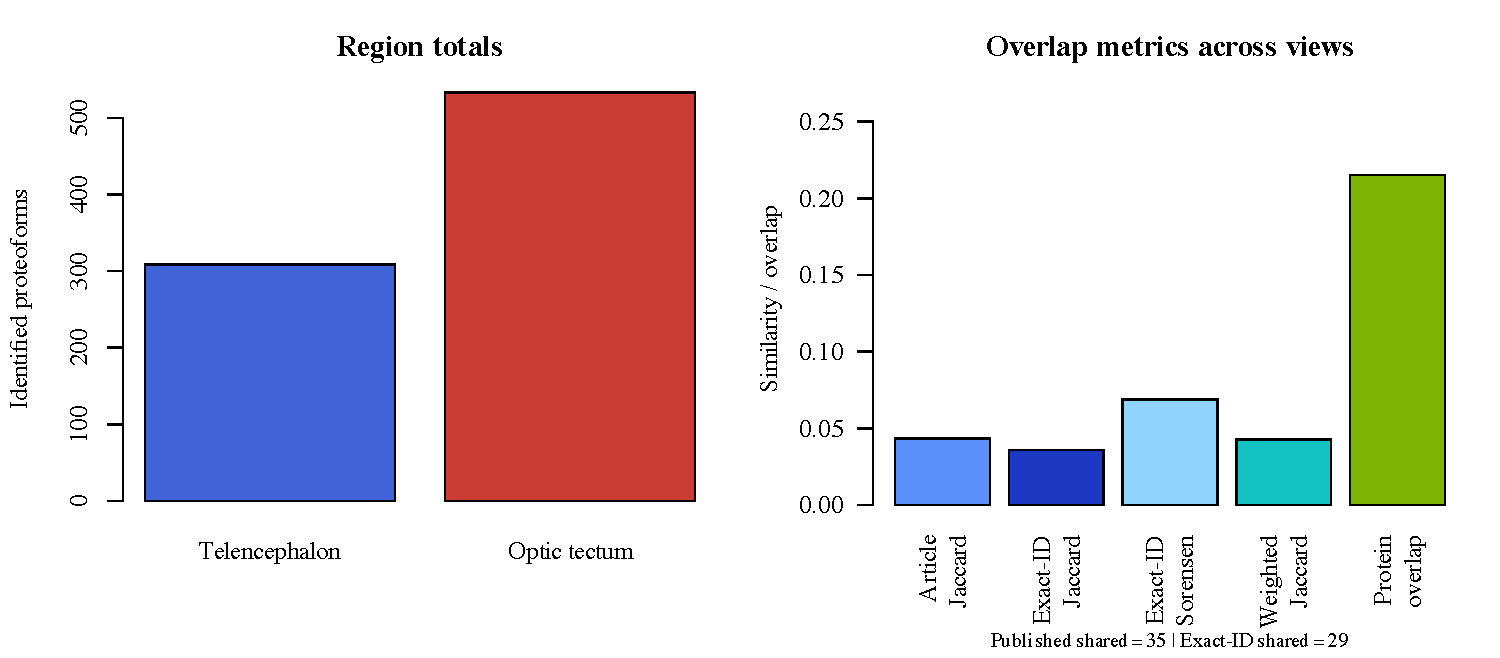
\includegraphics[width=0.97\linewidth]{../figures/fig1_region_overview.pdf}
    \caption{Regional totals and overlap metrics. The exact-ID source-table view is slightly stricter than the article aggregate, but both place telencephalon and optic tectum in the same low-overlap regime.}
    \label{fig:region-overview}
\end{figure}

\subsection{The source paper's biological interpretation becomes much stronger when expressed as an alignment problem}

A second substantive result is that this regional split is biologically organized in the expected direction. The curated marker panel is highly concentrated in the expected region. Telencephalon-associated markers contribute 23 matched counts and only 2 spillover counts, for an axis-level alignment fraction of 0.9200. Optic-tectum-associated markers contribute 102 matched counts and 1 spillover count, for an alignment fraction of 0.9903. Across the whole panel, the observed matched-region fraction is 0.9766. A naive baseline built only from the panel's own 25-versus-103 telencephalon/optic-tectum prevalence would predict 0.6904, so the observed alignment still exceeds that baseline by 0.2861. This matters because optic tectum contributes the larger raw proteoform total in the source study; the alignment result is therefore not just a restatement of optic-tectum abundance.

When those counts are written as a $2\times2$ table, the odds ratio is 1173 with an approximate 95\% confidence interval from 102.0 to 13{,}495.1, and the one-sided exact p-value is 5.12$\times10^{-22}$. The interval is necessarily wide because the off-diagonal cells are sparse, but even its lower bound still corresponds to a very large effect. The exact test is helpful, but the more intuitive story is the effect size: both functional axes sit far above the baseline expected from regional prevalence alone. The family-size-preserving randomization test makes the same point in a way that does not depend on asymptotic odds-ratio logic. Under 200{,}000 randomizations that preserved the nine family sizes and the global 25-versus-103 telencephalon/optic-tectum label totals, the null mean was only 88.4 matched counts and the 95th percentile was 95; none of those draws reached the observed 125 matched counts, giving a one-sided Monte Carlo upper bound of $5\times10^{-6}$.

These numbers do not imply that the entire proteome has been functionally classified. They mean something narrower and more useful: the particular marker proteoforms that the source article called biologically meaningful are overwhelmingly concentrated in the region whose known function they should support. That is the sense in which this paper turns a qualitative regional intuition into an explicit biological statement.

The count-based result is not hiding a family-composition problem. All 9 curated marker groups favor their expected region, the mean family-level matched share is 0.9826, the weakest family-level matched share is still 0.8750, and the corresponding one-sided sign-style probability under a 50:50 null is 0.001953. The conclusion is also stable across two stronger robustness moves that were not available in earlier versions of this paper. First, collapsing the curated panel to unique proteins still yields 28 matched proteins versus only 2 spillover proteins, for an alignment fraction of 0.9333, an odds ratio of 147.0, and a one-sided exact p-value of 3.02$\times10^{-5}$. A protein-collapsed family-size-preserving randomization tells the same story: the null mean is only 18.27 matched proteins, the 95th percentile is 22, and none of 200{,}000 draws reaches the observed 28 (Monte Carlo upper bound $=4\times10^{-5}$). Second, weighting the same panel by mean duplicate intensity yields a matched-region fraction of 0.9966, showing that the count-level result is not being driven by many weak spillover signals.

\begin{figure}[t]
    \centering
    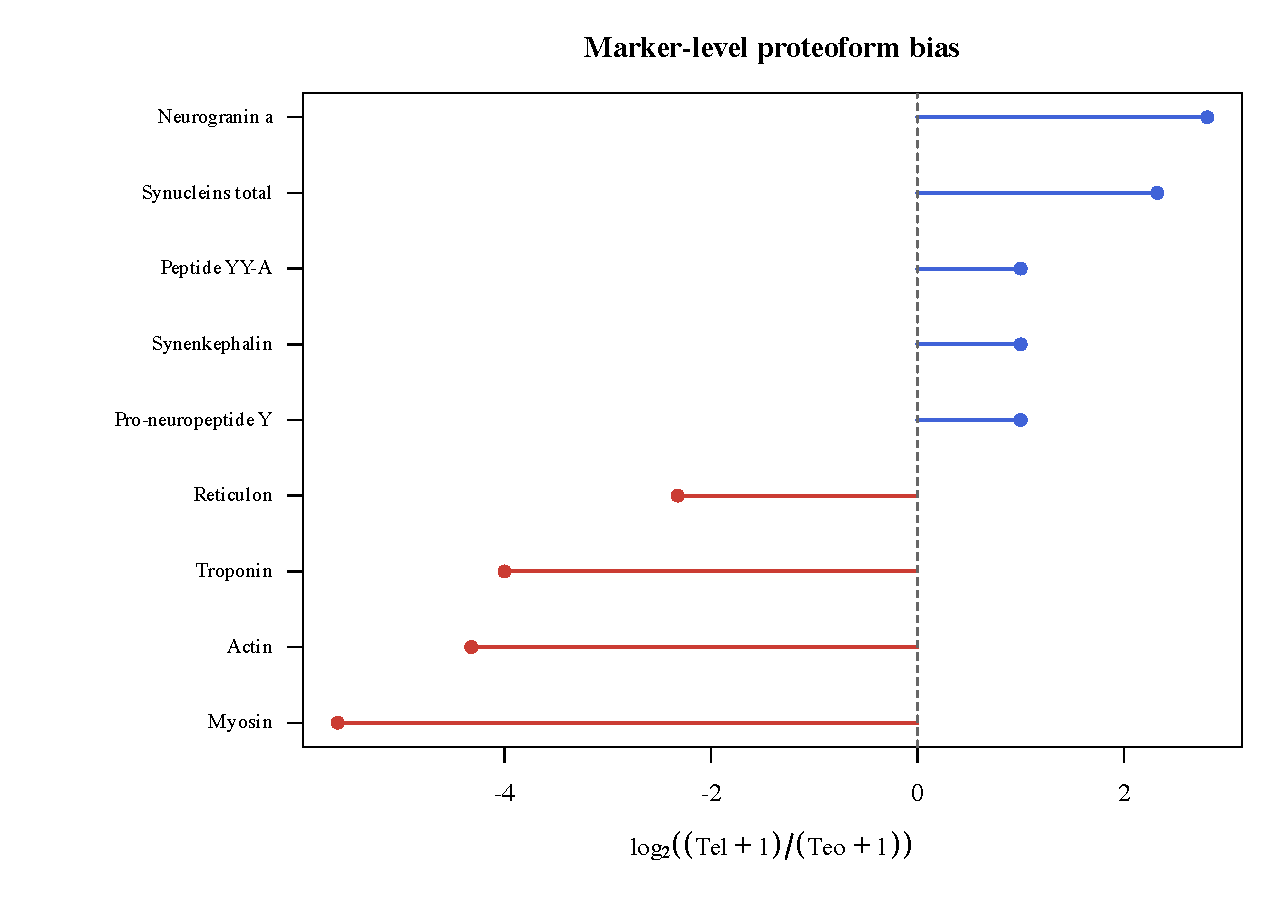
\includegraphics[width=0.90\linewidth]{../figures/fig2_marker_bias.pdf}
    \caption{Marker-level proteoform bias. Positive values favor telencephalon and negative values favor optic tectum.}
    \label{fig:marker-bias}
\end{figure}

\begin{figure}[t]
    \centering
    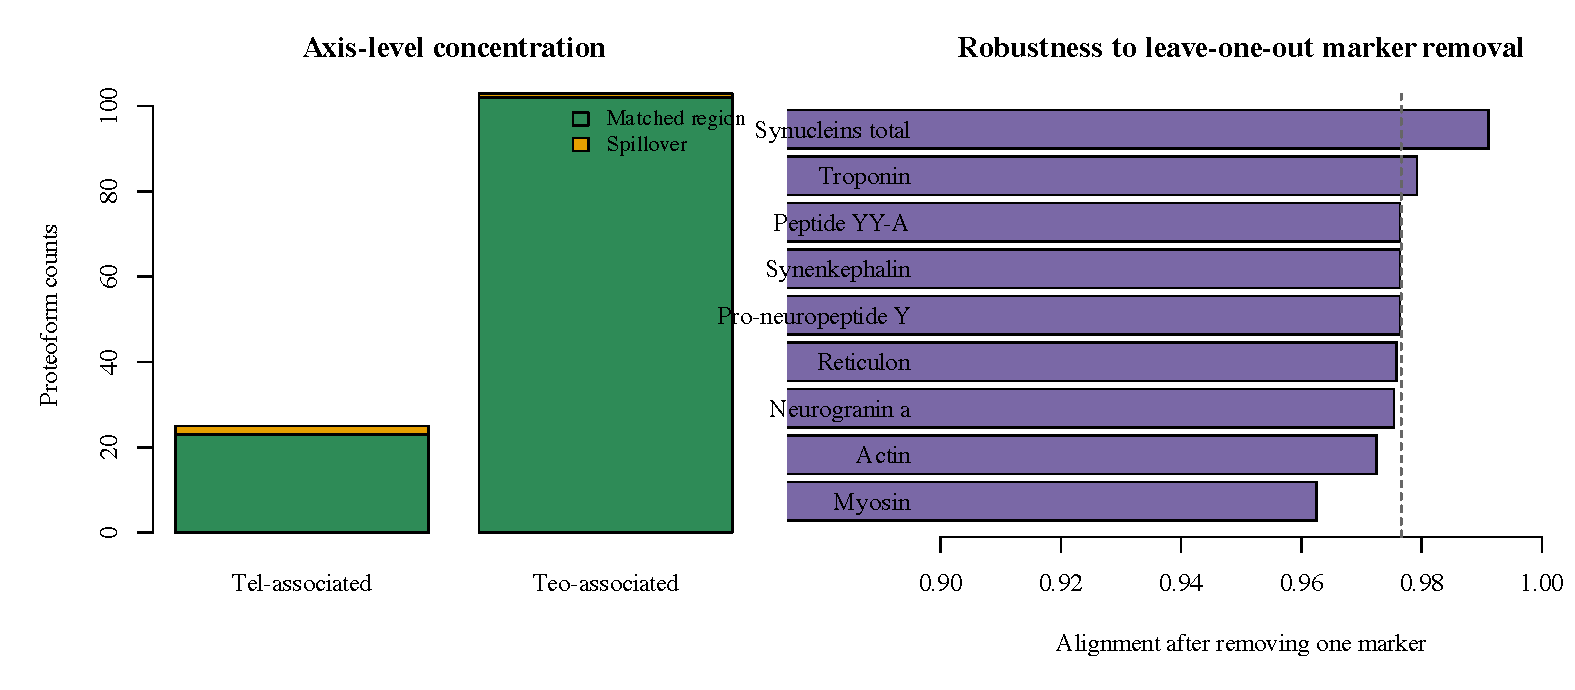
\includegraphics[width=0.97\linewidth]{../figures/fig3_axis_alignment.pdf}
    \caption{Axis-level concentration and robustness summaries. The overall alignment signal remains high after leave-one-out perturbation, after excluding motor families, after collapsing to proteins, and after weighting by mean duplicate intensity.}
    \label{fig:axis-alignment}
\end{figure}

\begin{table}[t]
\centering
\caption{Curated marker families used in the axis-alignment analysis. The released source tables now expose exact accession+proteoform members for each family in the local marker-membership file, but the biological framing still follows the source paper's named marker groups.}
\label{tab:markers}
\begin{tabular}{lrrl}
\toprule
Marker group & Tel & Teo & Interpretation \\
\midrule
Pro-neuropeptide Y & 1 & 0 & feeding-related neuropeptide signaling \\
Synenkephalin & 1 & 0 & affective signaling \\
Peptide YY-A & 1 & 0 & peptide hormone signaling \\
Neurogranin a & 6 & 0 & memory-linked synaptic signaling \\
Synucleins total & 14 & 2 & synaptic and mnemonic family \\
Reticulon & 0 & 4 & retinotectal organization \\
Myosin & 0 & 48 & motor machinery \\
Actin & 0 & 19 & cytoskeletal movement \\
Troponin & 1 & 31 & contraction-linked regulation \\
\bottomrule
\end{tabular}
\end{table}

\begin{table}[t]
\centering
\caption{Axis-level alignment compared with the naive baseline implied by regional prevalence.}
\label{tab:axisstats}
\begin{tabular}{lrrrr}
\toprule
Functional axis & Observed & Wilson 95\% CI & Baseline & Lift \\
\midrule
Telencephalon-associated & 0.9200 & 0.7503--0.9778 & 0.1875 & 0.7325 \\
Optic-tectum-associated & 0.9903 & 0.9470--0.9983 & 0.8125 & 0.1778 \\
\bottomrule
\end{tabular}
\end{table}

The leave-one-out analysis in Figure~\ref{fig:axis-alignment} also stays strong numerically: the matched-region fraction ranges only from 0.9625 to 0.9911 after removing any single marker family. The worst case comes from removing the large myosin group, yet even that stress test remains far above the naive prevalence baseline.

A second set of stress tests addresses the most obvious reviewer-style objections. If one, two, or three matched counts on each axis are pessimistically reassigned to spillover, the overall alignment fraction remains 0.9609, 0.9453, and 0.9297, respectively, while the odds ratio remains between 99.0 and 370.3. If the motor-associated myosin, actin, and troponin families are removed entirely to probe whether the optic-tectum signal is mainly a local contamination story, the remaining panel still aligns at 0.9310 with a Haldane-corrected odds ratio of 84.6. A lightweight composition guardrail points in the same direction: the released tables contain only 2 optic-tectum glial-support sentinels (GFAP and S100B) but 23 telencephalon myelin sentinels (MBPA/B) versus 3 in optic tectum. These checks do not eliminate missingness or purity concerns, but they show that the main regional-function signal is not being carried by a single fragile bookkeeping choice.

The review also asked for an independently curated panel that was not inherited from the source paper's own prose. Using adult zebrafish myelin markers from the zebrafish CNS myelin literature (PLP1b, MBPa, MBPb, MPZ/P0) together with adult optic-tectum radial-glia markers from the tectal precursor literature (GFAP, FABP7a, S100B) yields the same qualitative result. This independent panel contributes 32 matched counts and only 3 spillover counts, for an alignment fraction of 0.9143, an odds ratio of 73.3, and a one-sided exact p-value of $6.68\times10^{-4}$. After collapsing to proteins, the panel still aligns at 0.8750 with an odds ratio of 37.8 and $p = 0.00824$. The panel is smaller and more composition-oriented than the source paper's functional families, so it should not be read as a substitute for them. What it does show is that the regional separation signal is not resting entirely on the source paper's own choice of biologically favored markers.

\begin{table}[t]
\centering
\caption{Sensitivity checks requested by the external review. The motor-family exclusion uses a Haldane correction because one spillover cell is zero after exclusion.}
\label{tab:sensitivity}
\begin{tabular}{lrrr}
\toprule
Scenario & Alignment & Odds ratio & One-sided $p$ \\
\midrule
Observed panel & 0.9766 & 1173.0 & 5.12$\times10^{-22}$ \\
Shift 1 matched count per axis & 0.9609 & 370.3 & 2.01$\times10^{-19}$ \\
Shift 2 matched counts per axis & 0.9453 & 175.0 & 3.73$\times10^{-17}$ \\
Shift 3 matched counts per axis & 0.9297 & 99.0 & 3.93$\times10^{-15}$ \\
Exclude myosin, actin, troponin & 0.9310 & 84.6 & 6.32$\times10^{-4}$ \\
\bottomrule
\end{tabular}
\end{table}

\subsection{The pilot is PTM-rich and technically sensitive enough to justify proteoform-level interpretation}

The PTM follow-up contributes a third kind of knowledge, namely a disciplined negative result about what the public evidence does and does not support. The source article reports 807 identified proteoforms in total, of which 358 carry mass shifts and 211 are N-terminally acetylated. That means 44.36\% of the detected proteoforms belong to the modified subset and 58.94\% of the modified subset is N-terminally acetylated. These totals reinforce a simple point: the dataset is not just a protein list wearing different formatting. A large part of the biological signal lives at the proteoform level.

The source tables let us connect that PTM layer back to the regional marker analysis, but the reviewer-driven follow-up substantially changes how strongly we should read it. In the raw matched-marker counts, 14 of 23 telencephalon-matched proteoforms are N-terminally acetylated (0.6087), compared with only 16 of 102 optic-tectum-matched proteoforms (0.1569), for an unadjusted odds ratio of 8.36 and a one-sided exact p-value of $2.53\times10^{-5}$. That acetylation result remains significant after Holm correction across the two PTM screens in this paper (adjusted $p = 5.05\times10^{-5}$). By contrast, an exploratory ``other mass shift'' bucket shows 5/23 telencephalon-matched proteoforms and 20/102 optic-tectum-matched proteoforms, with no directional enrichment ($p = 0.508$).

The new detectability checks make the acetylation claim much more fragile. Among the acetylated matched-marker subsets, telencephalon rows are heavier (mean precursor mass 10{,}824.6 versus 6202.4; permutation $p = 3.05\times10^{-4}$), longer (mean residue span 106.1 versus 55.8; $p = 7.5\times10^{-5}$), and closer to the protein N terminus (mean first residue 1.0 versus 1.94; $p = 5\times10^{-6}$), while the mean duplicate intensity does not differ materially ($p = 0.417$). Once acetylation is rechecked in a coarse logistic sensitivity that adjusts for log precursor mass, span length, and first-residue position, the odds ratio falls to 2.94 with a 95\% confidence interval of 0.70--12.30 ($p = 0.140$). Restricting the analysis to matched-marker rows whose first residue lies at or within two positions of the N terminus removes the enrichment entirely (odds ratio 0.88, one-sided $p = 0.714$). The right reading is therefore no longer ``robust acetylation enrichment.'' It is that the public tables contain an interesting acetylation asymmetry, but that asymmetry is not stable once the available geometry and coverage proxies are taken seriously.

The technical-sensitivity numbers are also useful. The duplicate analyses yielded means of 232 proteoforms for telencephalon and 356 for optic tectum, corresponding to recovery fractions of 0.7508 and 0.6680 relative to the regional totals. The same released tables expose the incidence counts needed for Chao2 lower bounds: $q_1=154$, $q_2=155$ for telencephalon and $q_1=355$, $q_2=178$ for optic tectum. The single-run high-water mark was 418 proteoforms from an injected amount corresponding to roughly 250 cells in the source paper, or about 1.672 proteoforms per estimated sampled cell. That does not eliminate the pilot-study caveat, but it does explain why the study was able to expose biologically legible regional structure from very small samples while still leaving room for unseen-overlap sensitivity analyses.

\begin{table}[t]
\centering
\caption{Technical sensitivity values reported in the source study and extended with duplicate-incidence counts from the released source tables.}
\label{tab:technical}
\begin{tabular}{lrrrrrr}
\toprule
Region & Duplicate mean & Duplicate SD & CV & Recovery & $q_1$ & Chao2 lower bound \\
\midrule
Telencephalon & 232 & 28 & 0.1207 & 0.7508 & 154 & 385.5 \\
Optic tectum & 356 & 88 & 0.2472 & 0.6680 & 355 & 887.0 \\
\bottomrule
\end{tabular}
\end{table}

\begin{figure}[t]
    \centering
    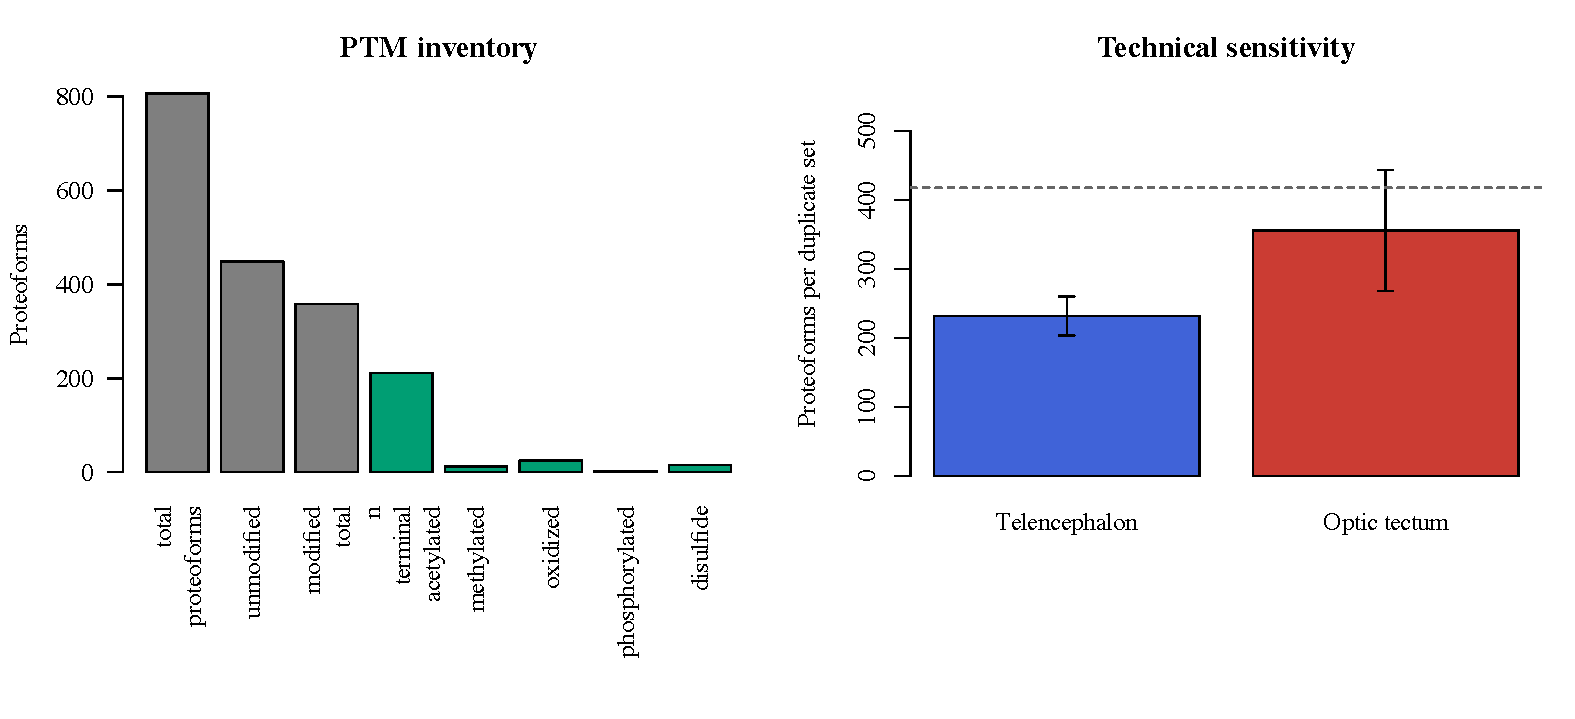
\includegraphics[width=0.97\linewidth]{../figures/fig4_ptm_and_sensitivity.pdf}
    \caption{PTM and missingness-sensitive follow-up analyses. Left: N-terminal acetylation is much more common in the telencephalon-matched marker subset than in the optic-tectum-matched subset. Right: duplicate-informed Chao2 sensitivity changes the exact-ID Jaccard modestly, but it never turns the regional split into a high-overlap regime.}
    \label{fig:ptm-sensitivity}
\end{figure}

\section{Discussion}

The main point is simple. Adult zebrafish telencephalon and optic tectum are not merely adjacent regions with somewhat different proteoform lists; they occupy sharply separated proteoform regimes whose dominant marker architecture follows known regional biology. The original study made that outcome plausible. The evidence assembled here makes it much harder to ignore. Once the named markers are rewritten as a matched-versus-spillover problem, the regional story is no longer a handful of appealing examples. The alignment fractions, odds-ratio interval, protein-collapsed robustness, intensity-weighted follow-up, and stress-test table all point in the same direction.

The biggest new factual gain over earlier versions of this note comes from the released Tel2 and Teo2 tables. They let us move from article-only overlap counts to exact accession+proteoform overlap, duplicate-incidence summaries, explicit marker-family membership tables, and a machine-readable evidence-traceability file. That extra layer matters because it exposes a small but real provenance wrinkle: the article reports 35 shared proteoforms, whereas the released exact-ID tables expose 29 exact matches. The new discrepancy diagnostic suggests that this is largely a representation issue rather than a biological contradiction. When bracketed PTM annotations and punctuation are stripped while accessions are retained, the shared count rises to 44, placing the published 35 between strict and relaxed matching rules. I therefore read the mismatch as a reminder that aggregate figure counts and released region tables are not always numerically identical, not as evidence that the present biological claim is an artifact of bookkeeping. The important point is that every public view still lands in the same regime: very low proteoform overlap and much higher protein overlap.

The supplementary workbook makes that provenance story cleaner as well. Its note sheet states that the public tables were identified in TopPIC at 1\% proteoform-spectrum-match FDR and 5\% proteoform-level FDR, with duplicate quantification performed in TopDiff, and its \texttt{Tel2} and \texttt{Teo2} sheets are exact copies of the standalone PRIDE tables used here. That does not prove the article's aggregate count of 35 shared proteoforms was produced under the same final aggregation logic, but it does make a simple table-side threshold mismatch less plausible than a representation or reporting difference.

The scope, however, remains narrow. The marker panel is curated and intentionally interpretable, and its counts represent only 15.20\% of the total regional count mass used here. The analysis therefore says less about the full latent structure of adult zebrafish brain proteomics than about one concrete point: this public pilot already supports a region-function proteoform axis that is sharper and more composition-aware than the original narrative presentation suggested. The technical replicate summaries remind us that this is still a pilot, not a large statistical atlas.

The new sensitivity checks sharpen that boundary in a useful way. Moving one to three matched counts per functional axis into spillover weakens the alignment effect, but it does not erase it. Likewise, excluding the three most obvious motor-associated families still leaves a strong optic-tectum-versus-telencephalon contrast in the remaining panel. The family-size-preserving randomization test is especially reassuring because it addresses the circularity objection in the units the paper actually uses: marker families. A null that preserves family sizes and the global telencephalon/optic-tectum label totals still centers around 88 matched counts, not 125, and none of 200{,}000 draws reaches the observed alignment. The duplicate-incidence calculations also push in the same direction: Chao2-style richness inflation lowers the exact-ID Jaccard if shared overlap is held fixed, and even the generous scaled-shared scenarios keep the overlap under 0.04. The first-order jackknife bound does the same. The new row-resampling and run-pair sensitivity files reach the same qualitative conclusion rather than rescuing a high-overlap story, and the prevalence-adjusted centered-Jaccard test shows that even the protein-collapsed overlap lies far below what the fixed margins would predict under independence. The minimal MNAR-style fill barely moves the weighted similarities. That means the current regional-separation claim survives modest curation perturbations, a plausible contamination objection, and more than one missingness model, even though it remains a public-table argument rather than a raw-feature validation study.

The orthogonal biological context also looks better after taking the review criticism seriously. The telencephalon side of the story is already well supported by behavioral and transcriptomic work on social orienting, learning, and memory \citep{stednitz2018social,reemst2023memory,pandey2023telencephalon}. On the optic-tectum side, the reticulon, myosin, actin, and troponin families fit a region that is visually driven, circuit-rich, and heavily involved in orienting transformations \citep{roeser2003tectum,orger2016visuomotor}. That does not prove every high-abundance motor-associated proteoform is a clean neuronal signal rather than a sampling or purity issue, but it makes the contamination-only explanation less attractive, especially once the non-motor panel still aligns strongly after exclusion and the released tables do not show a matching optic-tectum enrichment for the small glial/myelin sentinel screen. The new independent panel helps here as well. It is deliberately not a second copy of the source paper's own functional storytelling; it is a composition-oriented panel built from adult zebrafish myelin and adult optic-tectum radial-glia literature \citep{siems2021myelin,ito2010tectum}. The fact that it still separates the regions strongly suggests that the central result is broader than one hand-curated interpretive choice.

The PTM follow-up is also more informative than a simple ``there are many modified proteoforms'' statement, but it contributes by setting a boundary on current knowledge rather than by extending the positive claim. The raw matched-marker counts still show an acetylation asymmetry, and that asymmetry survives the limited Holm correction against the single exploratory non-acetyl bucket. Once the review forced us to model the public detectability proxies we actually have, however, the signal weakened substantially. The acetylated telencephalon-matched rows are heavier, longer, and more N-terminal than their optic-tectum counterparts, and the coarse covariate-adjusted logistic sensitivity no longer supports a confident region effect. Restricting to first-residue$\leq2$ rows removes the enrichment entirely. I therefore no longer read the acetylation contrast as a robust regional PTM program. The honest interpretation is narrower: the public tables contain a potentially interesting acetylation asymmetry, but the current release does not let us separate biology cleanly from proteoform geometry and coverage bias. That negative clarification is part of the contribution of the paper, because it prevents a fragile PTM hint from being mistaken for a settled biological program.

\subsection{Limits of inference}

This is not a raw-data reprocessing study, a new mass-spectrometry experiment, or a proteome-wide statistical atlas. It does not estimate region-wide significance for every detected proteoform, recover the full TopPIC workflow, or reinterpret unidentified mass shifts. Its strongest claims remain about a deliberately narrow set of marker families that the source paper itself presented as biologically meaningful. Even so, that is enough to support a useful statement about regional molecular organization, drawn from published counts, released region tables, and known regional function claims.

Several of the external review's requests still point to the same missing ingredient: richer feature-level detection histories. The released duplicate tables were enough for first-pass Chao2 and jackknife sensitivity, normalization checks, explicit marker-family traceability, and a limited PTM screen, but they still do not expose the full per-feature FDRs, localization confidence, charge-state resolution, or cross-region replicate incidence that a raw TopPIC export would provide \citep{choi2022toppic}. They also do not expose the higher-frequency incidence counts that would be required for iChao-style corrections. The current package therefore cannot adjudicate every possible redundancy or detectability objection. It can only show that several obvious objections fail to overturn the regional-function signal.

The literature on label-free normalization and missing-value handling is broader than what this tiny public design can support. EigenMS and later missingness-aware or imputation-oriented workflows were built for larger matrices and richer replication structures than two duplicate runs per region \citep{karpievitch2009eigenms,karpievitch2012missing,lazar2016missing}. For that reason this paper does not pretend to estimate a censoring model or an imputation pipeline from the released tables. Instead it treats blank cells as absent detections in the baseline analysis, reports several identifiable scaling schemes, and adds a minimal low-intensity-limit sensitivity so the reader can see how little the intensity-based overlaps move under a simple MNAR-style alternative.

The same ``do only what the public data can support'' rule also shapes the notation discussion. We now report that the relaxed overlap diagnostic is stable across three simple deterministic encodings, but that is still not the same thing as a full ProForma 2.0 implementation or a Proteoform Registry mapping \citep{leduc2018proforma}. Those standards are the right long-term answer when source strings and registry identifiers are available. Likewise, complementary bottom-up postquantification frameworks such as HiQuant are useful reference points for future cross-checking of proteoform stoichiometry, but they need peptide-level inputs that are outside the scope of this public top-down table release \citep{bryan2016hiquant}.

Those limits point directly to future work. The obvious next step is to extend the same analysis to the raw duplicate files now located on the PRIDE landing page together with the corresponding TopPIC feature exports or search intermediates, and then ask how much of the same function-legibility argument survives a proteome-wide treatment. Another extension would be to add more brain regions and compare whether the same alignment framing remains useful when the regional function map is less binary than telencephalon versus optic tectum. A third would be to formalize tissue-purity checks for the motor-associated families so that the contamination question can move from a stress test into a direct measurement. A fourth would be to connect this type of proteoform-specific auditability note more explicitly to the broader spatial-omics ecosystem: KRONOS and HEIST show what foundation-model scale looks like for spatial proteomics, imaging, and transcriptomics \citep{shaban2025kronos,madhu2025heist}, whereas this note occupies a complementary niche in which the priority is transparent proteoform-specific accounting over scale.

\section{Conclusion}

Adult zebrafish telencephalon and optic tectum are separated by distinct proteoform profiles, not merely by small shifts in abundance. The separating entries follow the expected biology of forebrain integration on one side and visuomotor architecture on the other, whereas the apparent acetylation asymmetry remains provisional. The proteoform layer therefore preserves a biological order that protein-level summaries partly obscure. In these data, two neighboring parts of the adult brain carry different molecular signatures of the work they do.


\bibliographystyle{plainnat}
\bibliography{references}

\appendix
\section{Reproducibility Appendix}

\subsection{Local files}

The package is backed by the source files in \texttt{data/}, the local analysis and figure scripts in \texttt{results/}, and the build scripts in \texttt{code/}. A minimal rebuild notebook is provided at \path{code/reproduce_tables_and_figures.ipynb}, and environment metadata is recorded in \path{code/environment_versions.json}.

\subsection{Formulas}

The main derived formulas are the Jaccard overlap, specialization fractions, marker-level stabilized log-bias, Wilson intervals for axis-level alignment fractions, an approximate odds-ratio interval for the $2\times2$ matched-versus-spillover table, an exact test on the same table, a prevalence-adjusted overlap-significance check based on the fixed-margin hypergeometric null, a two-run detectability correction based on duplicate rediscovery, and a conservative misidentification ceiling based on paired collapse of region-unique IDs.

\subsection{Extended computational details}

The main text reports only the quantities needed to follow the biology. The full computational path remains local and explicit. Exact-ID overlap is defined on accession-plus-proteoform pairs. The discrepancy diagnostic compares that strict unit with relaxed accession-plus-canonicalized-sequence matches that strip bracketed PTM annotations and punctuation while preserving accession identity. Protein-collapsed summaries merge rows at the protein identifier level. Abundance-weighted comparisons use mean duplicate intensities within each region and report both weighted Jaccard and Bray--Curtis similarity.

For prevalence-adjusted overlap, the observed telencephalon and optic-tectum margins are held fixed and the overlap count is evaluated against the fixed-margin hypergeometric null. The paper reports the observed Jaccard, the marginal-prevalence baseline under independence, the centered Jaccard, and the exact lower-tail $p$ value. Parallel summaries are also reported after collapsing the full dataset to gene symbols, so readers can see how much of the regional split depends on accession-resolved proteoform identity. For marker alignment, the analysis uses a matched-versus-spillover table together with Wilson intervals, an approximate odds-ratio interval, and an exact directional test. Family-size-preserving randomization keeps family sizes and the global telencephalon/optic-tectum label totals fixed while shuffling labels across the panel counts.

Missingness and abundance sensitivities are likewise kept local and inspectable. The duplicate \texttt{Match}/\texttt{No match} flags in the deposited spreadsheets provide the incidence counts used for Chao2 and first-order jackknife lower-bound richness calculations. Blank intensity cells are treated as absent detections in the baseline analysis, and the MNAR-style sensitivity fills missing exact IDs to half of the region-specific 5th-percentile or 10th-percentile nonzero intensity. Alternative abundance normalizations include per-run total-intensity scaling before duplicate averaging, region-level total-sum scaling, upper-quartile scaling, and median-ratio scaling on shared exact IDs.

The detectability bound uses the same duplicate structure in a different way. After collapsing each region to unique accession-plus-proteoform IDs, each exact ID is treated as detected in one run or both runs. Under a simple homogeneous two-run model, the duplicate-rediscovery counts give a region-specific per-run detection probability and therefore an estimated ``seen at least once'' probability for that region. The observed cross-region shared exact IDs are then divided by the product of those two region-level detection probabilities to estimate how much overlap could be hidden by uneven duplicate recovery alone. We also repeated that calculation after stratifying exact IDs by precursor-mass tertiles and by mean-intensity tertiles within each region. When a stratum contained no duplicate rediscovery, the stratum fell back to the corresponding region-level detectability estimate rather than generating an undefined correction. This remains intentionally simpler than a full hierarchical model, but it answers the reviewer's immediate question with quantities that are actually supported by the duplicate-labeled spreadsheets.

The misidentification sensitivity files are equally conservative. They do not claim to estimate the true false-discovery process. Instead, they ask how much the exact-ID Jaccard could rise if an equal fraction of region-unique exact IDs in both regions were actually paired representation or identification errors. The 1\% and 5\% scenarios track the PrSM- and proteoform-level FDR values reported in the source supplement. A second set of rows asks what error fractions would be required to raise the exact-ID Jaccard to 0.10 or all the way to the observed protein-level overlap.

\subsection{Accession conflicts, overlap statistics, and marker traceability}

When the same proteoform-like string appeared under more than one accession, the primary overlap analysis retained accession identity rather than collapsing immediately to gene or protein level. The reason is biological and practical: premature collapse can make distinct reported entries appear shared when the deposited spreadsheets still distinguish them. Protein-level summaries are therefore presented as sensitivity analyses, not as the primary unit of inference.

The prevalence-adjusted overlap statistics are reported for all three main representations. Under strict exact-ID matching, the observed Jaccard is 0.0360 against an independence baseline of 0.3152, yielding a centered Jaccard of $-0.2792$ with $p = 5.56\times10^{-183}$. Under canonicalized matching, the observed Jaccard is 0.0615 against an independence baseline of 0.3243, yielding a centered Jaccard of $-0.2627$ with $p = 5.01\times10^{-143}$. After protein collapse, the overlap rises to 0.2151, but still remains far below the protein-level independence baseline of 0.4280 with centered Jaccard $-0.2130$ and $p = 5.84\times10^{-33}$.

The marker-based interpretation is designed to remain externally auditable. The file \texttt{results/marker\_family\_membership.csv} links every curated family member to the source spreadsheet, row number, accession, proteoform string, matching rule, and matched-versus-spillover assignment. The file \texttt{results/motor\_family\_breakdown.csv} further expands the myosin and troponin families into accession-level entries together with simple annotation classes, so the contamination question can be inspected directly. The file \texttt{data/evidence\_traceability.json} mirrors the marker mapping at the claim level so that each headline statement in the paper can be traced back to a concrete local artifact.

\subsection{Scope note}

The computation uses values recoverable from the published article and the deposited region spreadsheets. It does not claim a full raw-data reprocessing pipeline.

\subsection{Canonicalization and missing-intensity note}

Canonicalization is used only as a discrepancy diagnostic, not as the paper's primary biological unit. The strict analysis unit remains accession plus proteoform string. In the diagnostic view, bracketed PTM annotations, punctuation, and non-sequence characters are removed before matching. The file \texttt{results/canonicalization\_examples.csv} now separates each example into sequence core, modification tokens, residue window, and canonicalized sequence so that the discrepancy can be inspected in a ProForma-oriented way \citep{leduc2018proforma,leduc2022proforma2}. We do not emit full ProForma 2.0 strings for the whole dataset because the deposited spreadsheets do not expose the localization metadata needed for exact standard-compliant serialization. Blank intensity cells in the deposited spreadsheets are treated as absent detections in the baseline analysis and contribute zero intensity; the reviewer-driven MNAR sensitivity file records two low-intensity-limit alternatives.

\subsection{Reproducibility metadata}

The package records software versions and platform metadata in \path{code/environment_versions.json}. For review, the exact code and derived-table bundle accompanies the manuscript in \texttt{code/}, \texttt{results/}, and \texttt{data/}. The notebook at \path{code/reproduce_tables_and_figures.ipynb} gives a compact path through the main tables and figures. The same metadata file records the public project repository URL, but no archival DOI has yet been minted for this specific example package.

\subsection{Detectability-adjusted acetylation model}

The covariate-adjusted acetylation analysis is intentionally simple. It uses the matched marker rows only. One model codes region as the binary outcome and uses acetylation status, log precursor mass, sequence span length, and first-residue position as predictors, with the continuous covariates standardized before fitting. The inverse model codes acetylation as the outcome and region as the main predictor while keeping the same covariates. The goal is not to claim a complete model of proteoform detectability. It is to ask whether the apparent acetylation asymmetry survives once the strongest public-table correlates of detectability are placed in the same coarse model. It does not. A second analysis then restricts the rows to first residue $\leq 2$ as a stricter N-terminal geometry screen.

\subsection{Public provenance note}

The journal supplement records that the deposited spreadsheets were generated with 1\% PrSM FDR and 5\% proteoform-level FDR in TopPIC and quantified across duplicate runs in TopDiff. The same supplement also embeds \texttt{Tel2} and \texttt{Teo2} sheets that match the standalone PRIDE XLSX files exactly. The PRIDE landing page lists the four raw duplicate files, but this package does not claim a raw-file reprocessing study.

\subsection{Exact rebuild path}

The package can be rebuilt locally with:
\begin{verbatim}
cd examples/codex-zebrafish-brain-paper-14rounds
./code/build_inputs.sh
./code/build_paper.sh
\end{verbatim}

The analysis step should regenerate the summary metrics, exact-ID overlap files, marker-membership and robustness files, the run-pair and bootstrap sensitivity files, and the figure assets. The paper step should regenerate \texttt{paper/main.pdf}.

\subsection{Marker-panel curation rule}

The marker panel is intentionally conservative. A family enters the panel only if the source proteomics paper names it in the biological interpretation of telencephalon or optic tectum and if that interpretation can be connected to established zebrafish regional function in the cited background literature. The curated counts and family labels are materialized in \texttt{data/curated\_evidence.json}, while the corresponding exact source-table members, row numbers, and matching rules appear in the marker-membership CSV and the traceability JSON.

\subsection{Why the curation unit is still a marker family}

The deposited region spreadsheets do expose reusable machine-readable proteoform IDs, and this version of the package takes advantage of that fact. Even so, the strongest biological interpretation in the paper still runs through the marker families named in the original article rather than through a full proteoform-by-proteoform atlas. That is deliberate. The exact-ID files strengthen traceability and missingness sensitivity, but the functional claim remains aligned with the families that the original paper itself foregrounded as biologically interpretable.

\subsection{Leave-one-out and sensitivity files}

The full leave-one-out table and the reviewer-driven sensitivity scenarios are saved as \path{results/leave_one_out_alignment.csv} and \path{results/sensitivity_scenarios.csv}. The main text and Figure~\ref{fig:axis-alignment} summarize the same robustness story.

\subsection{Claim-to-evidence ladder}

\begin{table}[ht]
\centering
\small
\caption{Main claims, supporting evidence, and corresponding limits.}
\label{tab:evidenceladder}
\begin{tabular}{p{0.26\linewidth}p{0.33\linewidth}p{0.28\linewidth}}
\toprule
Claim & Evidence & Main limit \\
\midrule
Proteoform-level regional separation & Article Jaccard 0.0434, exact-ID Jaccard 0.0360, occupancy-adjusted Jaccard 0.0432, 5\% misidentification ceiling 0.0540, protein overlap 0.2151 & Public tables, not raw-feature reprocessing \\
Functional markers align with expected region & Axis alignment, exact test, sign check, leave-one-out table, protein collapse, intensity weighting & Curated marker panel only \\
PTM layer contains a suggestive but unstable acetylation asymmetry & Unadjusted acetylation 14/23 versus 16/102; detectability and covariate sensitivity files & Public tables do not separate biology cleanly from geometry/coverage bias \\
Package improves auditability & Local code, figures, manifests, exact marker membership, and evidence traceability & Does not replace the source experiment \\
\bottomrule
\end{tabular}
\end{table}

\subsection{Claim-to-file map}

The repository-level package keeps the full claim-to-file map in the local README and machine-readable manifests. In-paper, the important point is simply that every headline result in the main text is backed by a corresponding local CSV/JSON artifact plus the figure that summarizes it.


\end{document}
